\begin{minipage}{0.3\textwidth}
\section*{P-A*mbush}

\begin{itemize}
\item If agent $i$ is the closest one to the goal, it
could be beneficial to make $i$ perform the path computing
first.

\item P-A$^*$ambush incorporates a strategy that decides
which agent calculates its path first.

\item We propose the real distance as a good strategy, because
the positions of the agents are a very general and intuitive
property that defines the advantage of an agent over another
one.

\end{itemize}

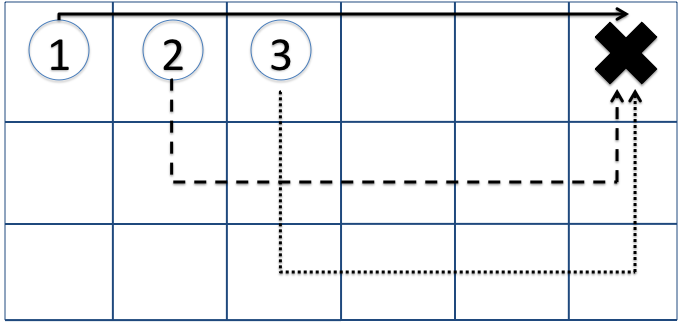
\includegraphics[width=0.48\textwidth]{figures/ambush_grid.png}
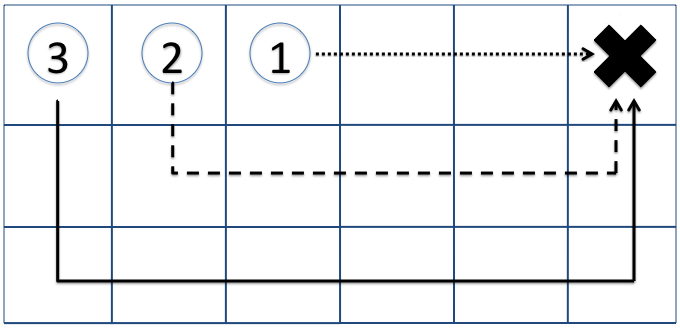
\includegraphics[width=0.48\textwidth]{figures/priorities_grid.png}
\end{minipage}